\documentclass{beamer}

\usepackage[utf8]{inputenc}
\usepackage{amsmath,amsthm}
\usepackage{amssymb}
\usepackage{bbm}
\usepackage{amsfonts}
\usepackage{wasysym}

\usepackage{xcolor}
\definecolor{lightred}{RGB}{209,105,81}
\definecolor{lightgreen}{RGB}{58,181,75}
\definecolor{thickblue}{RGB}{5,43,108}
\definecolor{lightblue}{RGB}{0,153,228}

\usepackage{graphicx}
\graphicspath{ {./graphics/} }

\usepackage{enumitem}
\usepackage{pifont}


\setbeamertemplate{frametitle}[default][center]
\setbeamertemplate{navigation symbols}{}
\setbeamerfont{footline}{series=\bfseries}
\setbeamertemplate{footline}[page number]

\usepackage{tikz}
\newcommand{\topline}{%
  \tikz[remember picture,overlay] {%
    \draw[gray, thick] ([xshift=1cm,yshift=-1.2cm]current page.north west)
             -- ([xshift=-1cm,yshift=-1.2cm,xshift=\paperwidth]current page.north west);}}
             
             
%Information to be included in the title page:
\title{\color{lightred}\textbf{Transportation of New York}}
\author{Xinyu Chen}

\vspace{-10em}
% \institute{Overleaf}
\date{ }



\begin{document}

\begin{frame}

\begin{center}
    {\color{lightred}\Large\textbf{Transportation of New York}}
    
    \vspace{2em}
    
    \textbf{\color{thickblue}Xinyu Chen}
\end{center}

% \titlepage
\vspace{2em}

\centering

\includegraphics[scale=0.2]{graphics/citibike_travel.png}
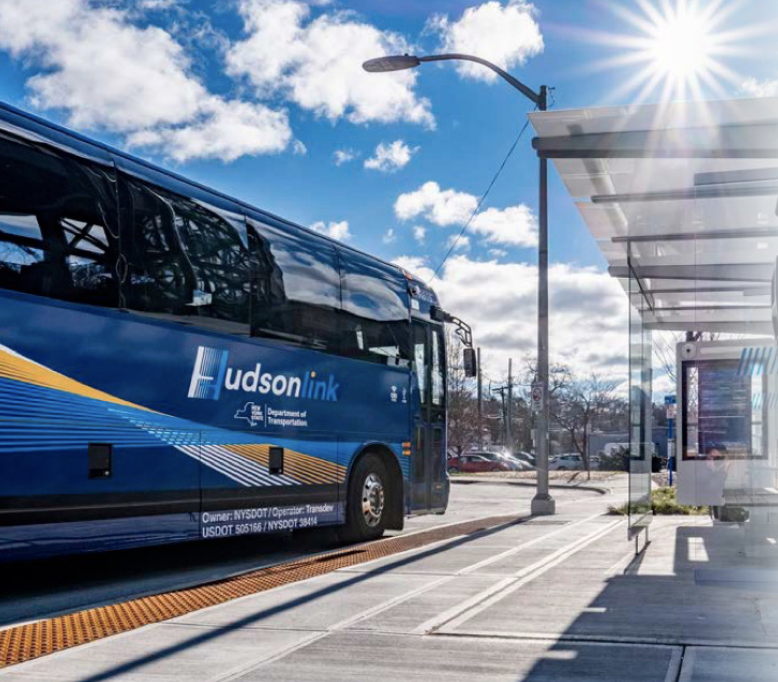
\includegraphics[scale=0.165]{graphics/nyc_bus.png}
    
\end{frame}


\begin{frame}
\frametitle{\color{lightred}\textbf{Outline}}
\topline
{\color{black}
\begin{itemize}[label=\ding{212}]
\item Introduction
\item Modal share
\item Transportation systems
\begin{itemize}[label=\ding{48}]
    \item {\small{Transit system}}
    \item {\small{Shared mobility}}
    % \item Private car
    % \item Pedestrian infrastructure
\end{itemize}
\item GHG emissions
\item Traffic safety
% \item Comparing New York to Montreal
\item Travel behavior trend
\item Uniqueness of transport
\item Reference
% \item A research article
\end{itemize}
}
\end{frame} 


\begin{frame}

\frametitle{\color{lightred}\textbf{Introduction}}
\topline

\begin{columns}
\begin{column}{0.45\textwidth}
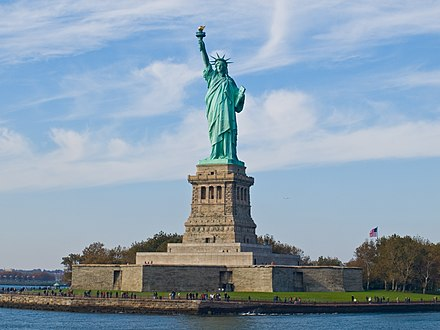
\includegraphics[scale=0.3]{graphics/lady_liberty.jpg}

\vspace{0.5em}

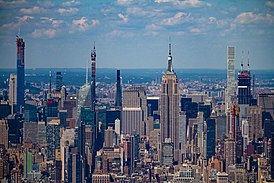
\includegraphics[scale=0.48]{graphics/Midtown_Manhattan.jpg}

\end{column}
\begin{column}{0.55\textwidth}

\textbf{\color{thickblue}New York City}

\footnotesize

- The \textbf{\color{lightred}most populous city} in the US

- The \textbf{\color{lightred}most densely populated major city} in the US

\centering
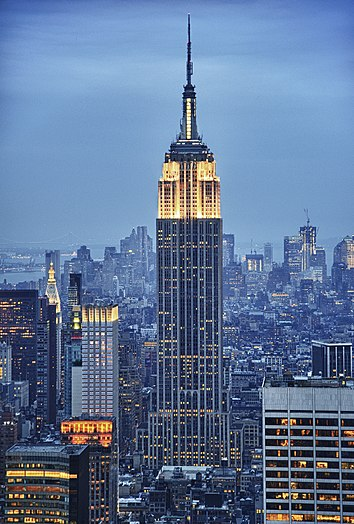
\includegraphics[scale=0.28]{graphics/Empire_State_Building.jpg}

\end{column}
\end{columns}

\end{frame}


\begin{frame}
\frametitle{\color{lightred}\textbf{Introduction}}
\topline

\textbf{\color{thickblue}New York City}

{\footnotesize

- \textbf{\color{black}784 $\text{km}^{2}$} \hspace{1em} - Population: \textbf{8.34 million} (2019)
}

\vspace{1em}
{\centering\includegraphics[scale=0.2]{graphics/nyc_map.png}
}

\vspace{1em}

\textbf{\color{thickblue}Montreal}

{\footnotesize

- \textbf{\color{black}432 $\text{km}^{2}$} \hspace{1em} - Population: \textbf{4.20} (2019)
}


\end{frame}


\begin{frame}
\frametitle{\color{lightred}\textbf{Introduction}}
\topline

\begin{columns}
% \hspace{-2em}
\begin{column}{0.8\textwidth}
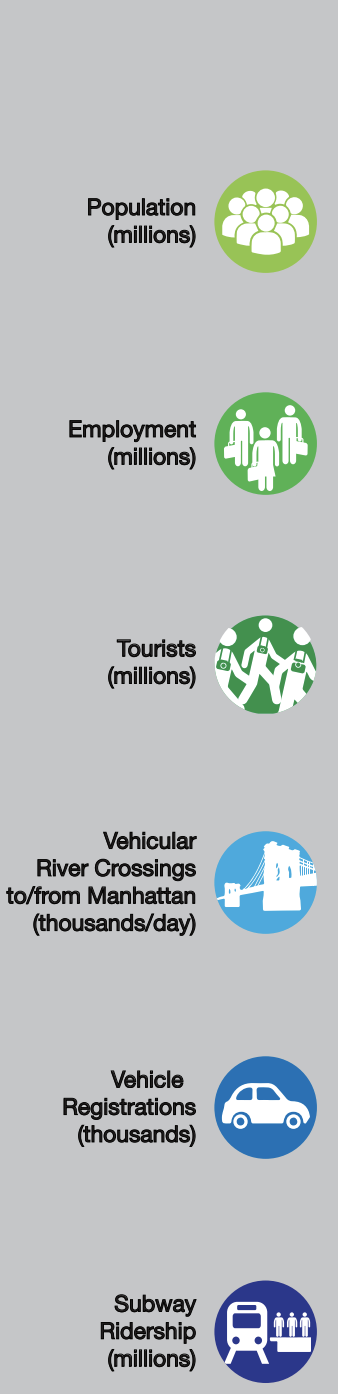
\includegraphics[scale=0.27]{graphics/nyc_mobility_stat1.png}\hspace{-0.4em}
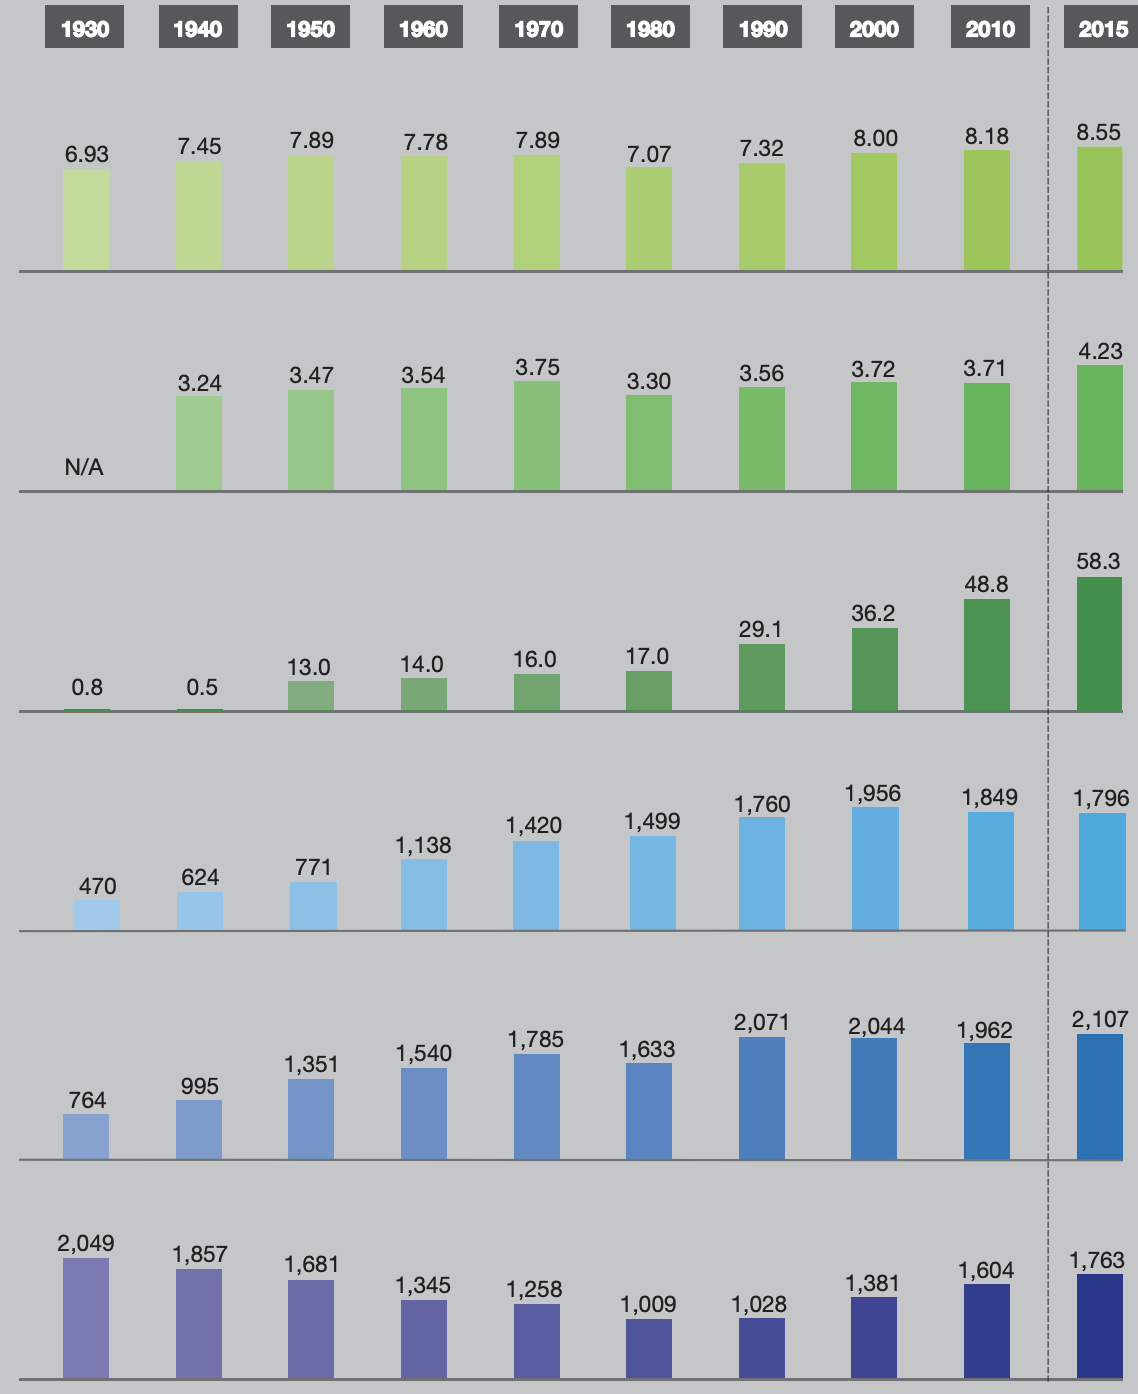
\includegraphics[scale=0.27]{graphics/nyc_mobility_stat2.png}
\end{column}

\hspace{-5em}
\vspace{-15em}
\begin{column}{0.4\textwidth}

% \textbf{\color{thickblue}New York City}

\textbf{\color{lightgreen}Growth in 1980-2010:}
\begin{itemize}[label=\ding{212}]\footnotesize
    \item Population: \textbf{16\%}
    \item Employment: \textbf{12\%}
    \item Tourism: \textbf{187\%}
    \item Subway rideship: \textbf{59\%}
\end{itemize}
\end{column}
\end{columns}

\end{frame}


\begin{frame}
\frametitle{\textbf{\color{lightred}Modal share of NYC residents}}
\topline

\begin{columns}
\begin{column}{0.5\textwidth}

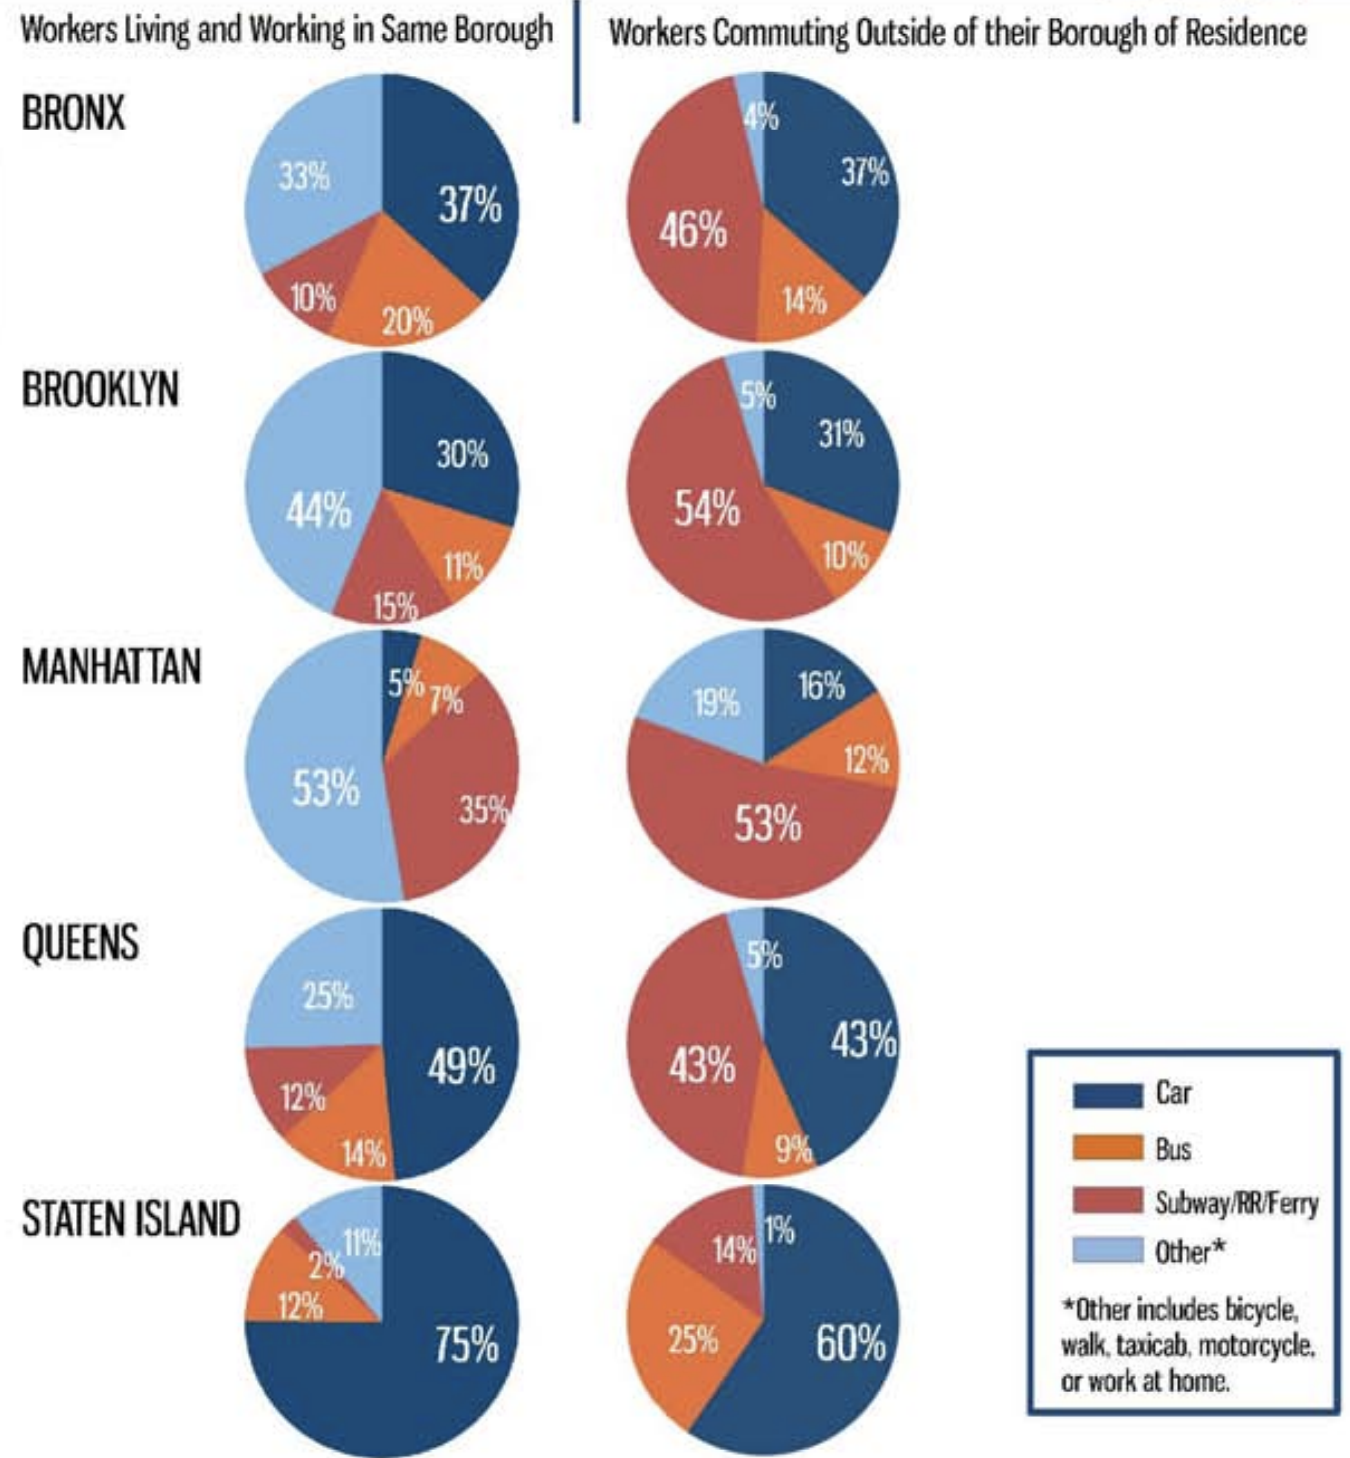
\includegraphics[scale=0.25]{graphics/modal_share.png}

\end{column}
\begin{column}{0.5\textwidth}
\textbf{\color{thickblue}Findings}

\vspace{1em}
\footnotesize

\begin{itemize}[label=\ding{48}]
    \item Subway/Railroad/Ferry is the largest mode among workers commuting outside of their borough of residence, except on Staten Island.
    \item In Queens and Staten Island, the plurality of workers use cars for commuting.
\end{itemize}
\end{column}
\end{columns}

\end{frame}



\begin{frame}

\frametitle{\color{lightred}\textbf{Transit system}}
\topline

\begin{columns}
\begin{column}{0.4\textwidth}
\textbf{\color{thickblue}Subway in NYC}

{\footnotesize

\begin{itemize}[label=\ding{212}]
    \item {\color{lightblue}6,600 subway cars}
    \item {\color{lightblue}472 subway stations}
    \item Daily rideship: $\approx$ {\color{lightblue}5.5 million}
    \item Annual rideship:
    \begin{itemize}[label=\ding{48}]
        \item {\color{lightblue}1.76 billion} (2015)
        \item {\color{lightblue}1.70 billion} (2019)
    \end{itemize}
\end{itemize}
}

\textbf{\color{thickblue}Subway in Montreal}

{\footnotesize

\begin{itemize}[label=\ding{212}]
    \item {\color{lightblue}68 subway stations}
    \item Daily rideship: $\approx$ {\color{lightblue}1.4 million} (Q4 2018)
    \item Annual rideship: {\color{lightblue}0.35 billion} (2016)
\end{itemize}
}

\end{column}

\hspace{-3em}

\begin{column}{0.6\textwidth}
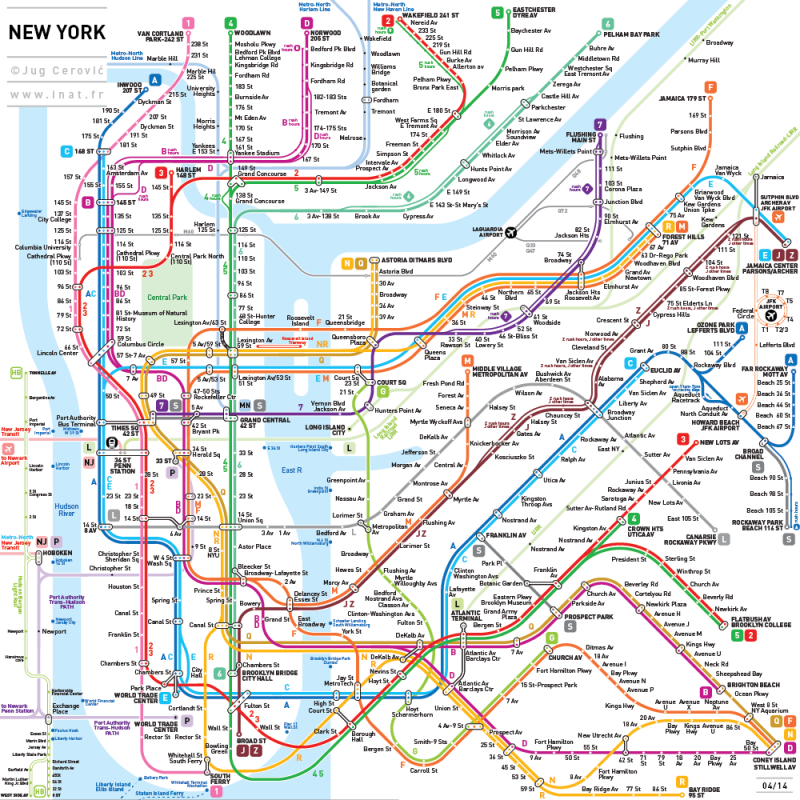
\includegraphics[scale=0.3]{graphics/subway_map.png}
\end{column}

\end{columns}

\end{frame}


\begin{frame}

\frametitle{\color{lightred}\textbf{Transit system}}
\topline
\begin{columns}
\begin{column}{0.45\textwidth}
\textbf{\color{thickblue}Bus in NYC}
{\footnotesize
\begin{itemize}[label=\ding{48}]
    \item {\color{lightblue}5,927 vehicles} in the bus fleet
    \item All 100\% accessible to riders with disabilities
    \item {\color{lightblue}234 local bus routes}
    \item {\color{lightblue}20 Select Bus Service routes}
    \item {\color{lightblue}73 express routes}
    \item Annual rideship:
    \begin{itemize}[label=\ding{48}]
        \item {\color{lightblue}651 million} (2015)
        \item {\color{lightblue}557 million} (2019)
    \end{itemize}

\end{itemize}
}

\textbf{\color{thickblue}Bus in Montreal}
{\footnotesize
\begin{itemize}[label=\ding{48}]
    \item {\color{lightblue}1,449 vehicles} in the bus fleet
    \item {\color{lightblue}220 bus lines}
    \item Annual rideship:
    \begin{itemize}[label=\ding{48}]
        \item {\color{lightblue}234 million} (2015)
        \item {\color{lightblue}223 million} (2017)
    \end{itemize}

\end{itemize}
}

% \includegraphics[scale=0.5]{x}
\end{column}

\hspace{-4em}

\begin{column}{0.55\textwidth}
\begin{columns}
\begin{column}{0.27\textwidth}
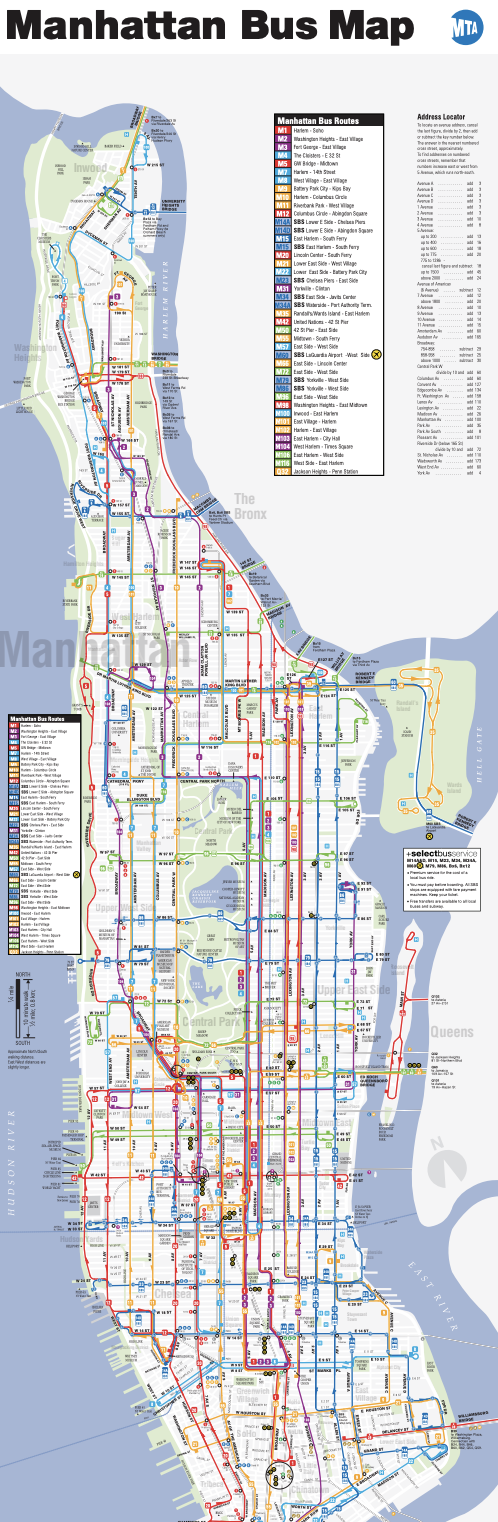
\includegraphics[scale=0.25]{graphics/manhattan_bus_map.png}
\end{column}

\hspace{-3em}

\begin{column}{0.27\textwidth}
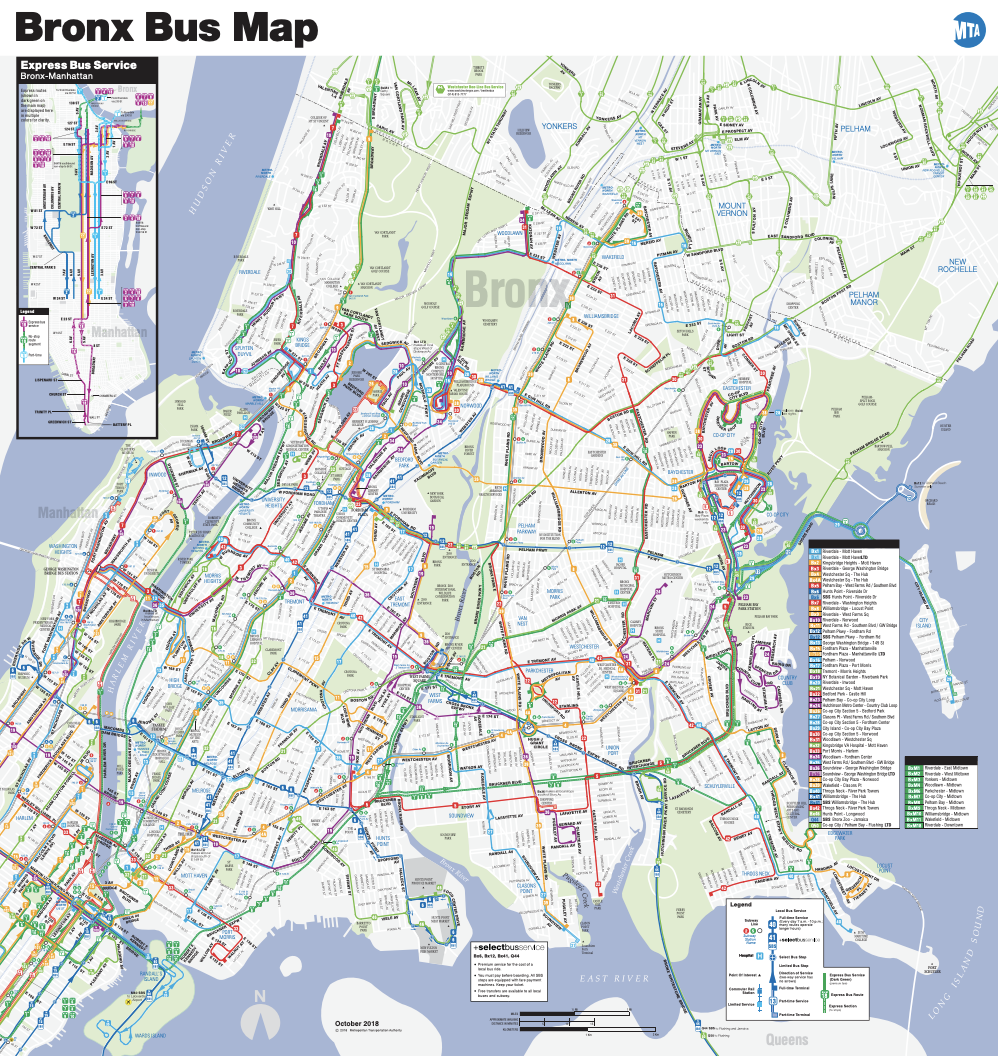
\includegraphics[scale=0.18]{graphics/bronx_bus_map.png}
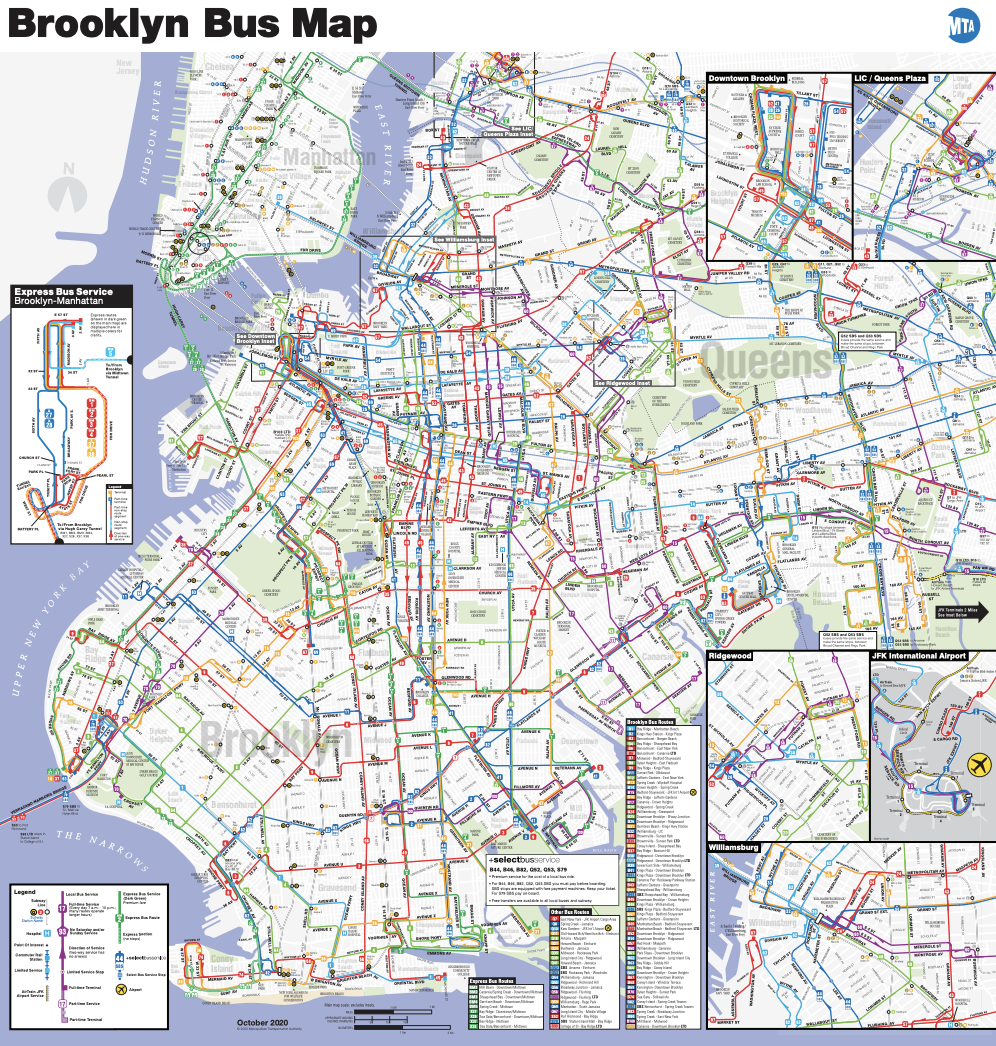
\includegraphics[scale=0.18]{graphics/brooklyn_bus_map.png}
\end{column}
\end{columns}
\end{column}

\end{columns}

\end{frame}




\begin{frame}

\frametitle{\color{lightred}\textbf{Shared mobility}}
\topline

\centering
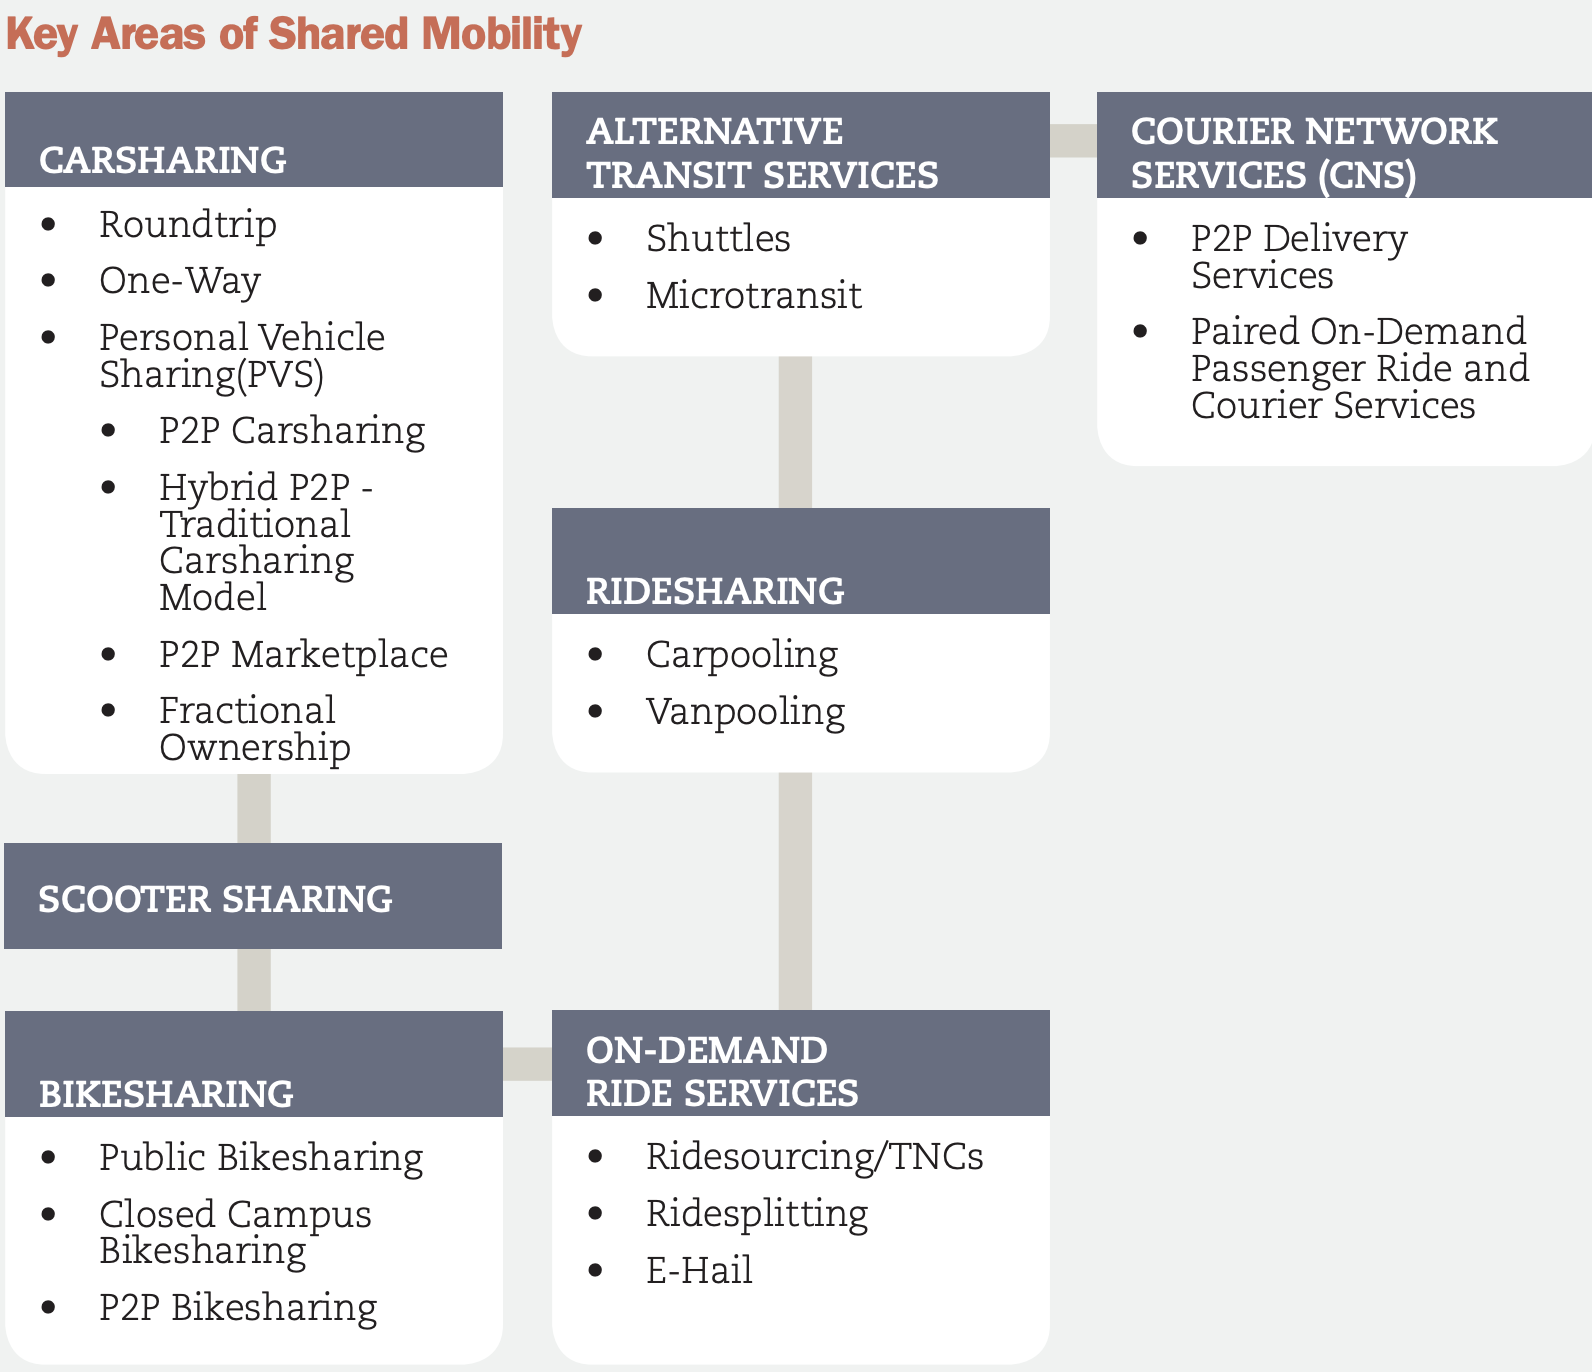
\includegraphics[scale=0.34]{graphics/shared_mobility.png}

    
\end{frame}


\begin{frame}

\frametitle{\color{lightred}\textbf{Shared mobility}}
\topline

\textbf{\color{thickblue}Ride-hailing}

\vspace{1em}

\includegraphics[scale=0.2]{graphics/taxi_pickup1.png}
\includegraphics[scale=0.2]{graphics/taxi_pickup2.png}

\vspace{1em}

\footnotesize

Over the past 4 years,

- {\color{lightblue}ride-hailing apps have grown from 0 to 15 million trips per month}

- {\color{lightblue}taxi usage has only declined by around 5 million trips per month}

\end{frame}



\begin{frame}
\frametitle{\color{lightred}\textbf{Shared mobility}}
\topline

\textbf{\color{thickblue}Citi Bike}

\vspace{1em}

\begin{columns}
\begin{column}{0.65\textwidth}
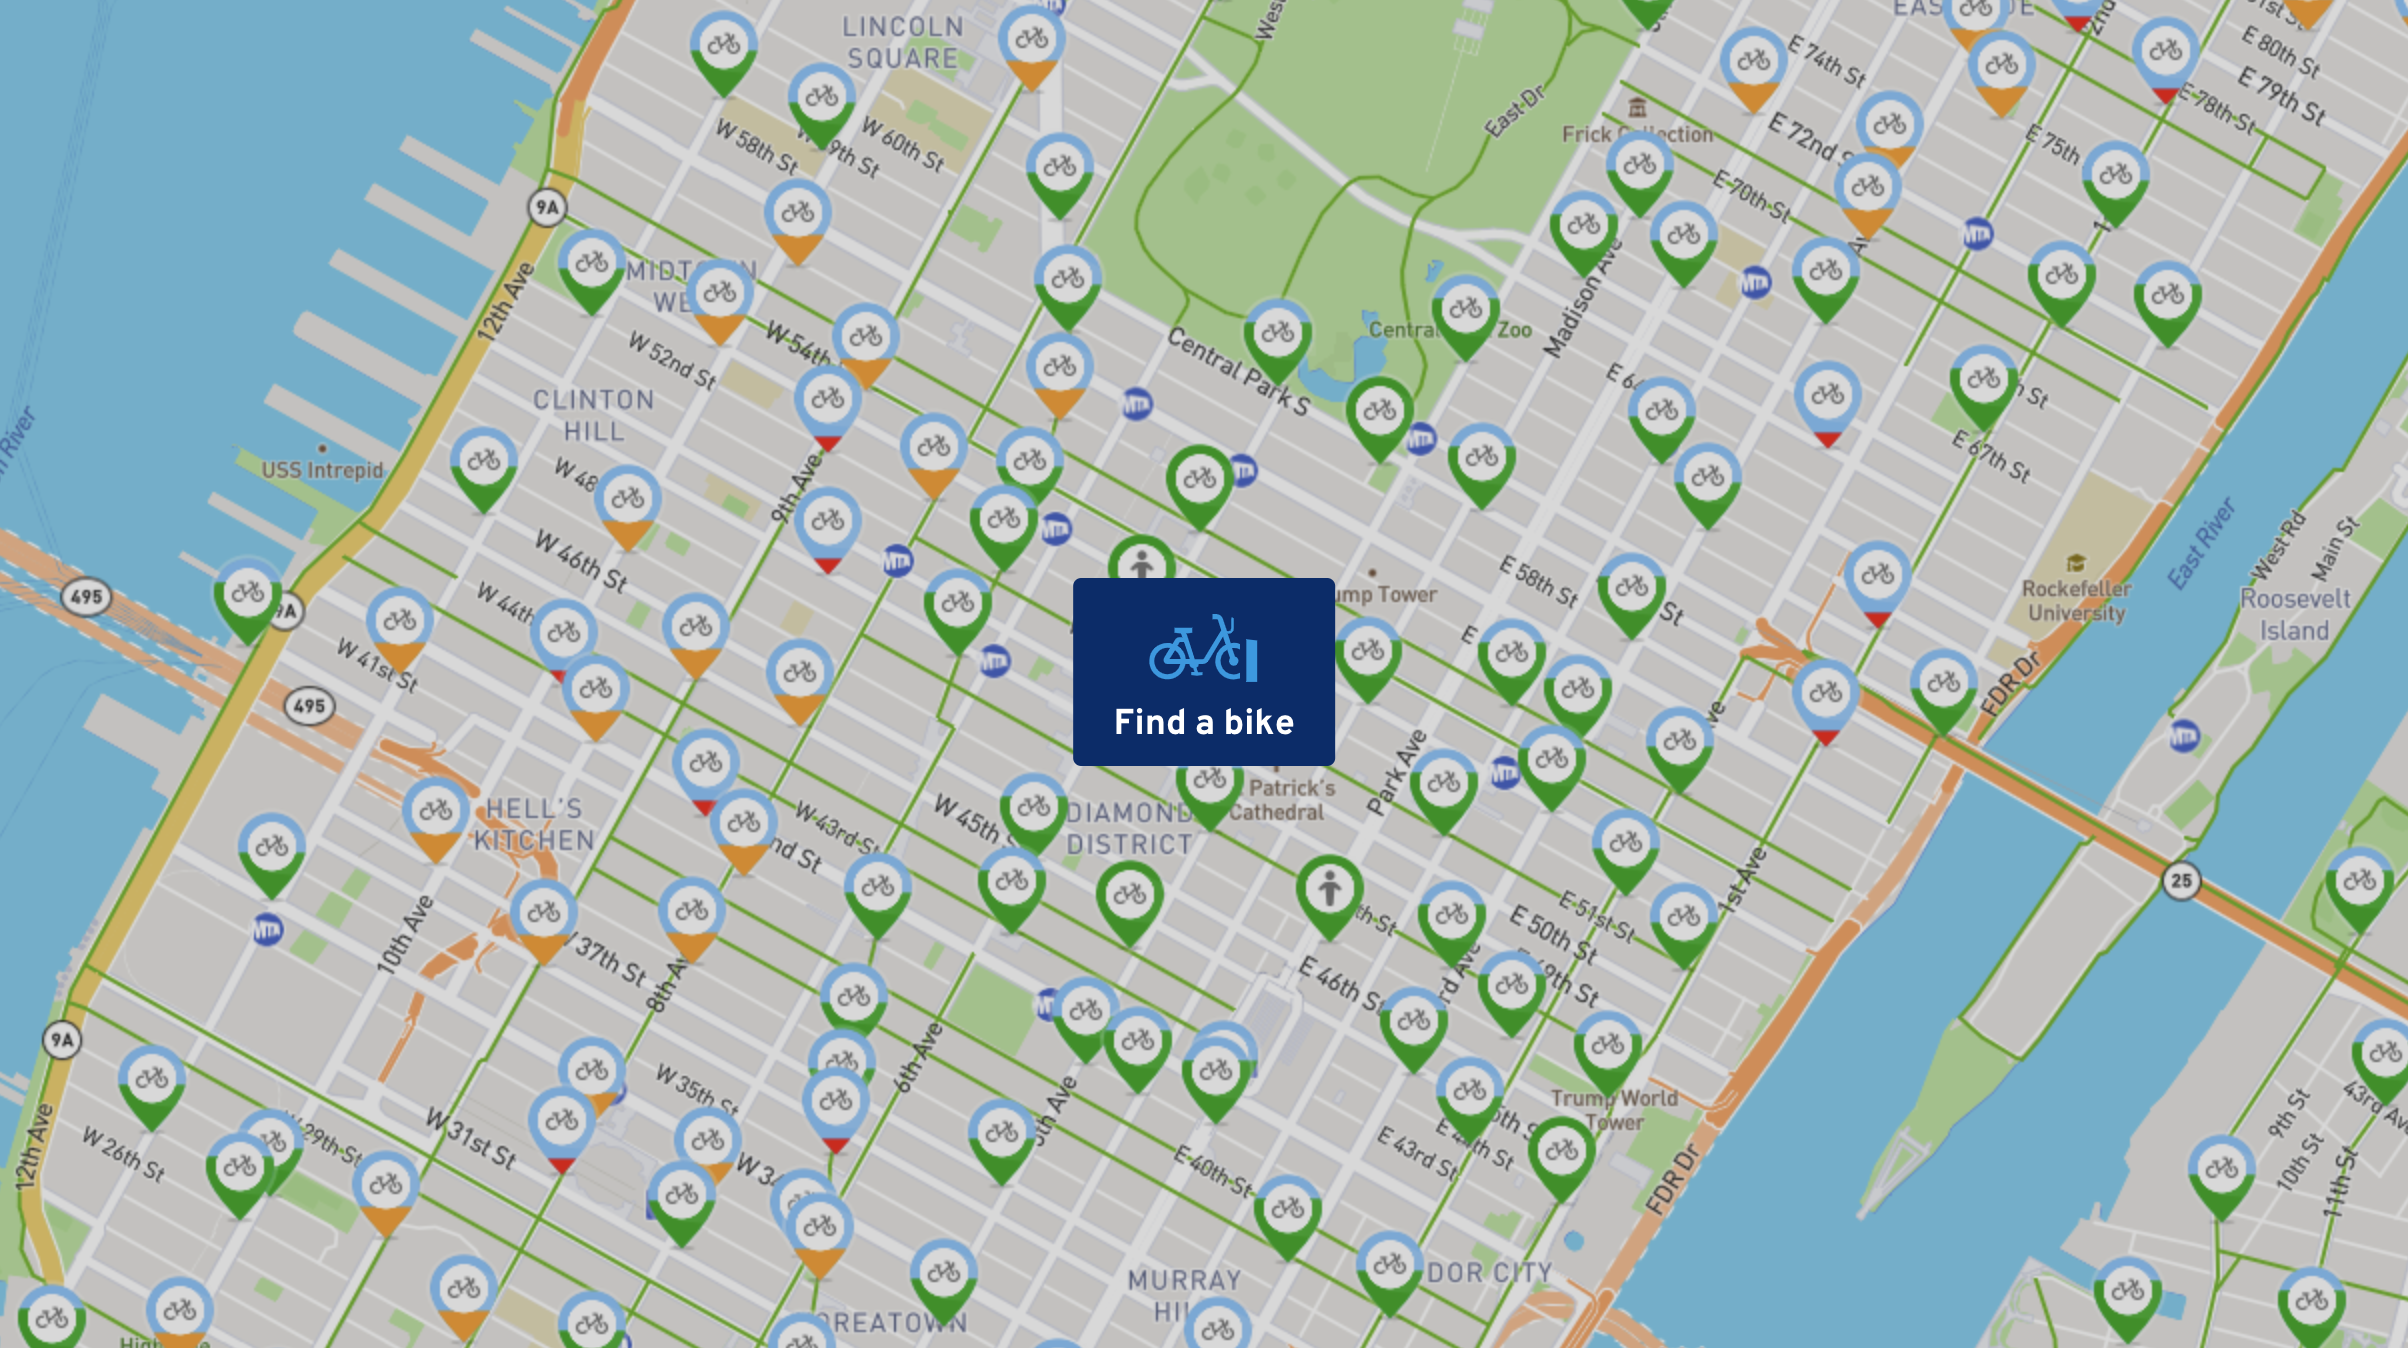
\includegraphics[scale=0.14]{graphics/find_a_bike.png}

\vspace{1em}

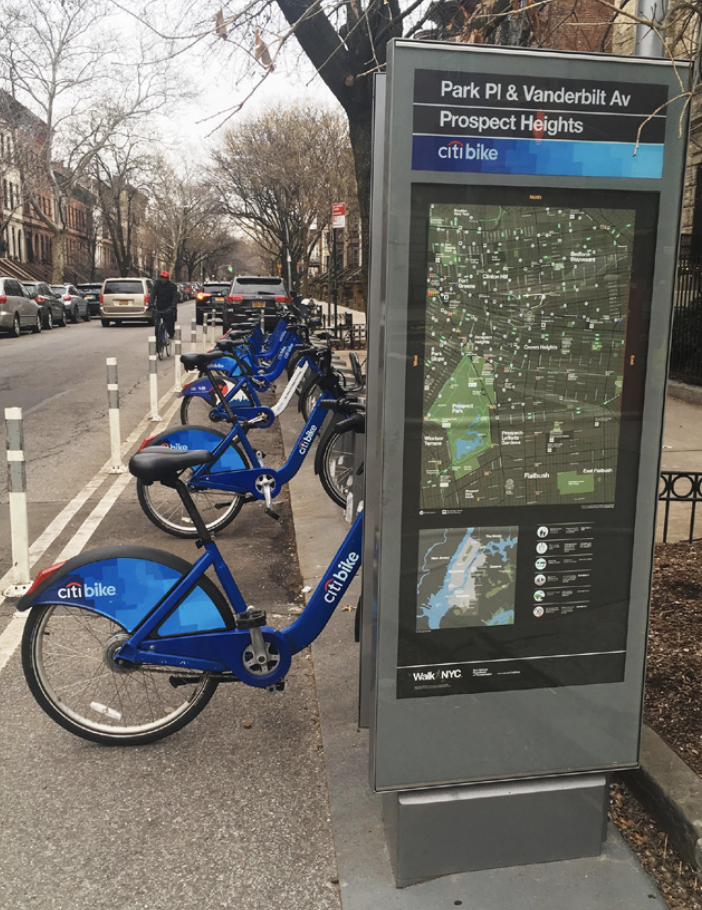
\includegraphics[scale=0.22]{graphics/citibike.png}\hspace{1em}
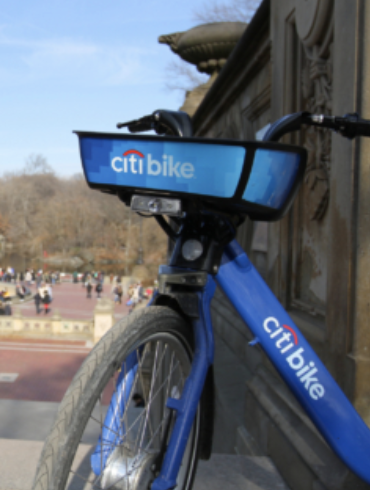
\includegraphics[scale=0.41]{graphics/citibike2.png}
\end{column}

\hspace{-5em}

\begin{column}{0.45\textwidth}
{\footnotesize
\begin{itemize}[label=\ding{212}]
    \item The {\color{lightblue}nation's largest bike share} program.
    \item {\color{lightblue}15,000 bikes}
    \item {\color{lightblue}1,000+ stations}
\end{itemize}
}

\vspace{1em}

\textbf{\color{thickblue}Bikes in Montreal}
{\footnotesize
\begin{itemize}[label=\ding{212}]
    \item {\color{lightblue}540+ stations}
\end{itemize}
}
\end{column}
\end{columns}
    

\end{frame}


\begin{frame}
\frametitle{\color{lightred}\textbf{Shared mobility}}
\topline

\textbf{\color{thickblue}Citi Bike}

\vspace{1em}

\begin{columns}
\begin{column}{0.5\textwidth}
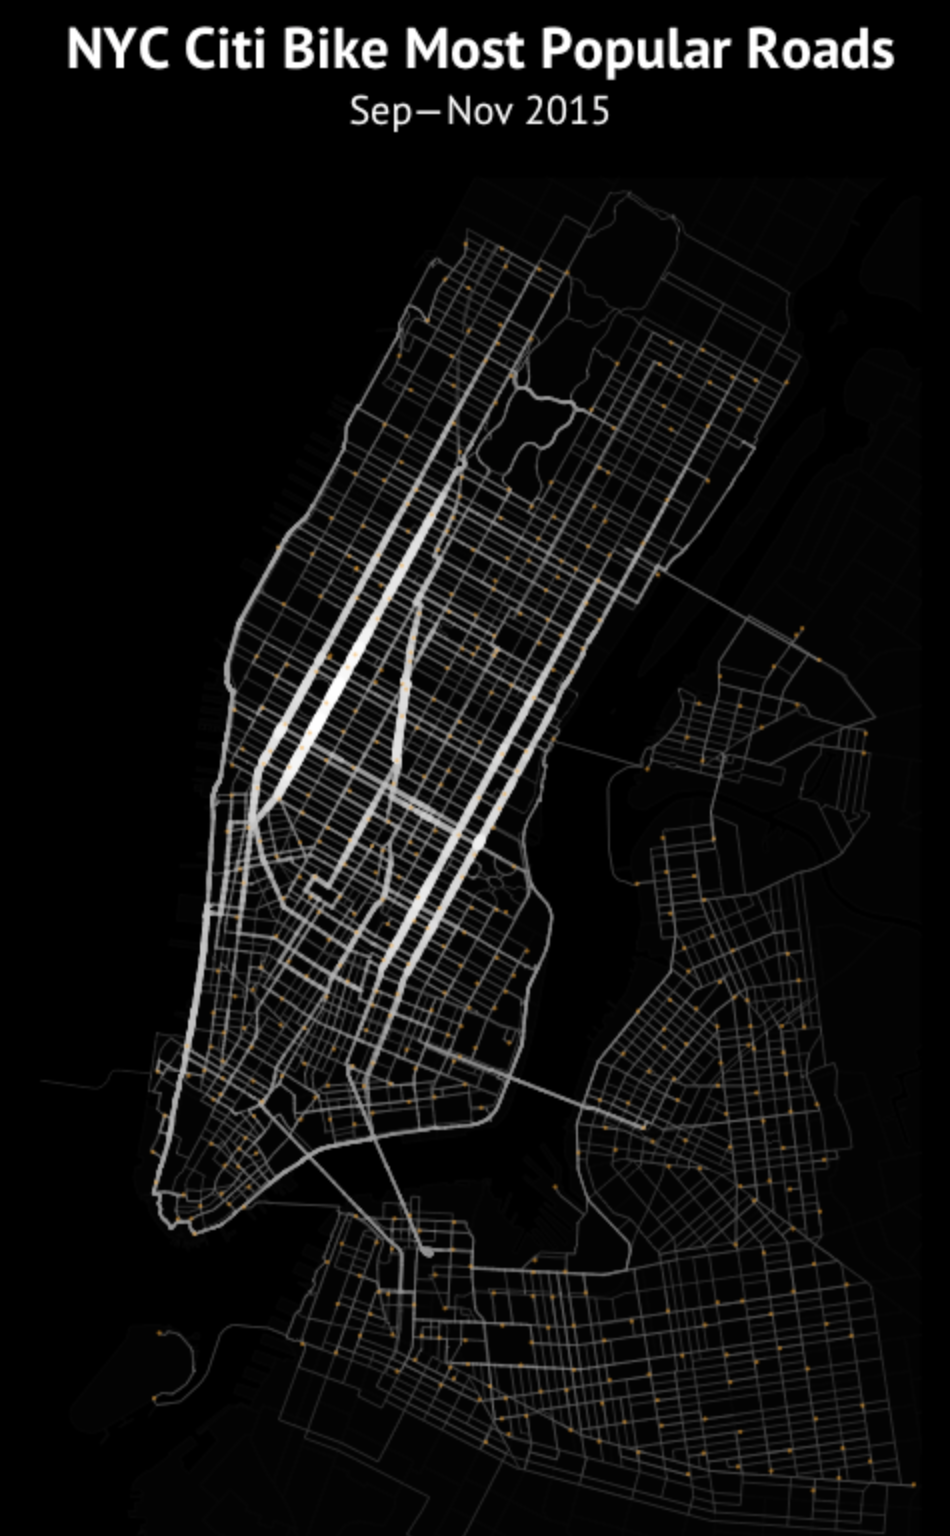
\includegraphics[scale=0.25]{graphics/citibike_popular_road.png}

\end{column}

\hspace{-5em}

\begin{column}{0.5\textwidth}

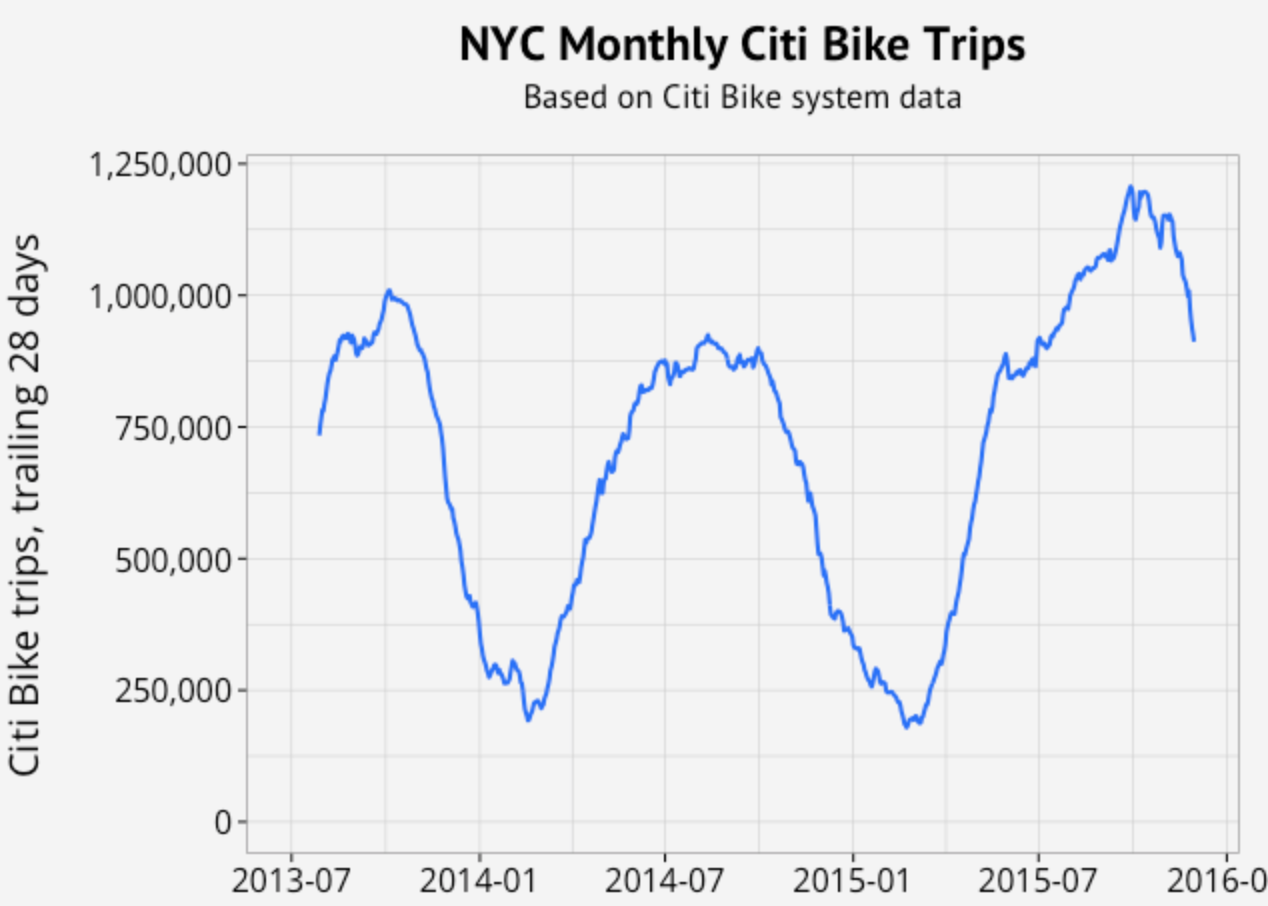
\includegraphics[scale=0.25]{graphics/citibike_monthly_trips.png}

\vspace{1em}

\footnotesize
\begin{itemize}[label=\ding{212}]
    \item {\color{lightblue}dramatically fewer rides during the cold winter months}
    \item {\color{lightblue}1,000,000+ rides in some months}
    % \item {\color{lightblue}The August 2015 increase in rides corresponds to the system’s first major expansion}
\end{itemize}
\end{column}
\end{columns}

\end{frame}


\begin{frame}
\frametitle{\color{lightred}\textbf{GHG emissions}}
\topline

\begin{columns}
\begin{column}{0.7\textwidth}
\centering
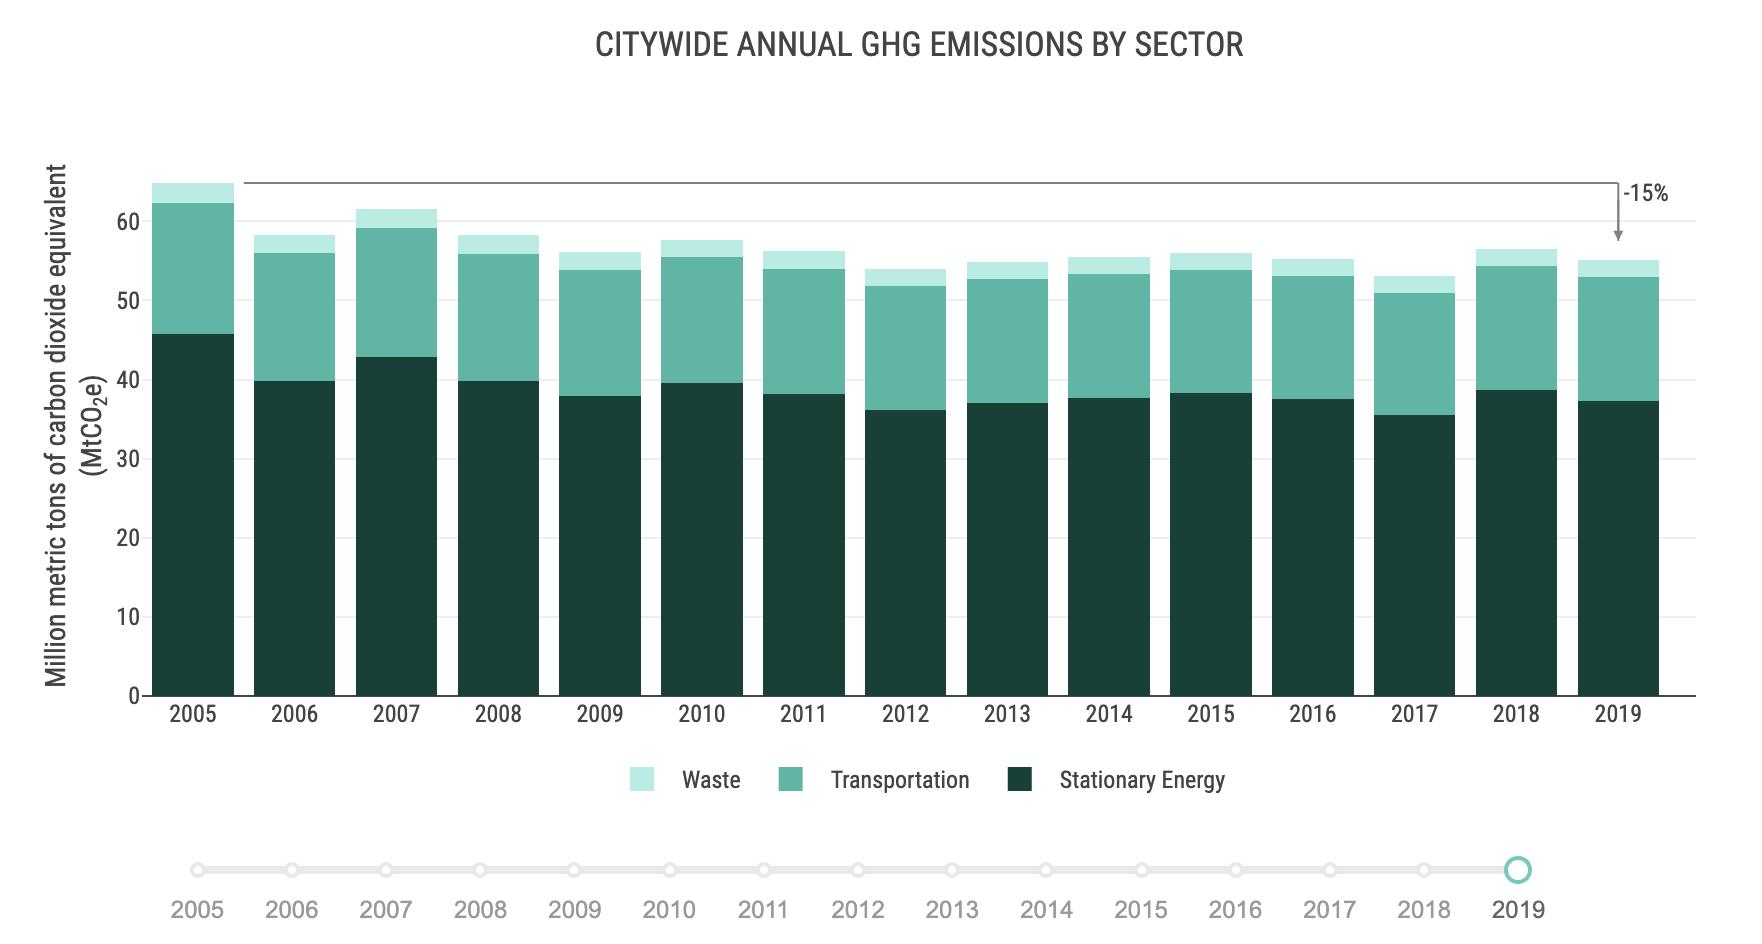
\includegraphics[scale=0.24]{graphics/nyc_ghg.png}

\hspace{1em}

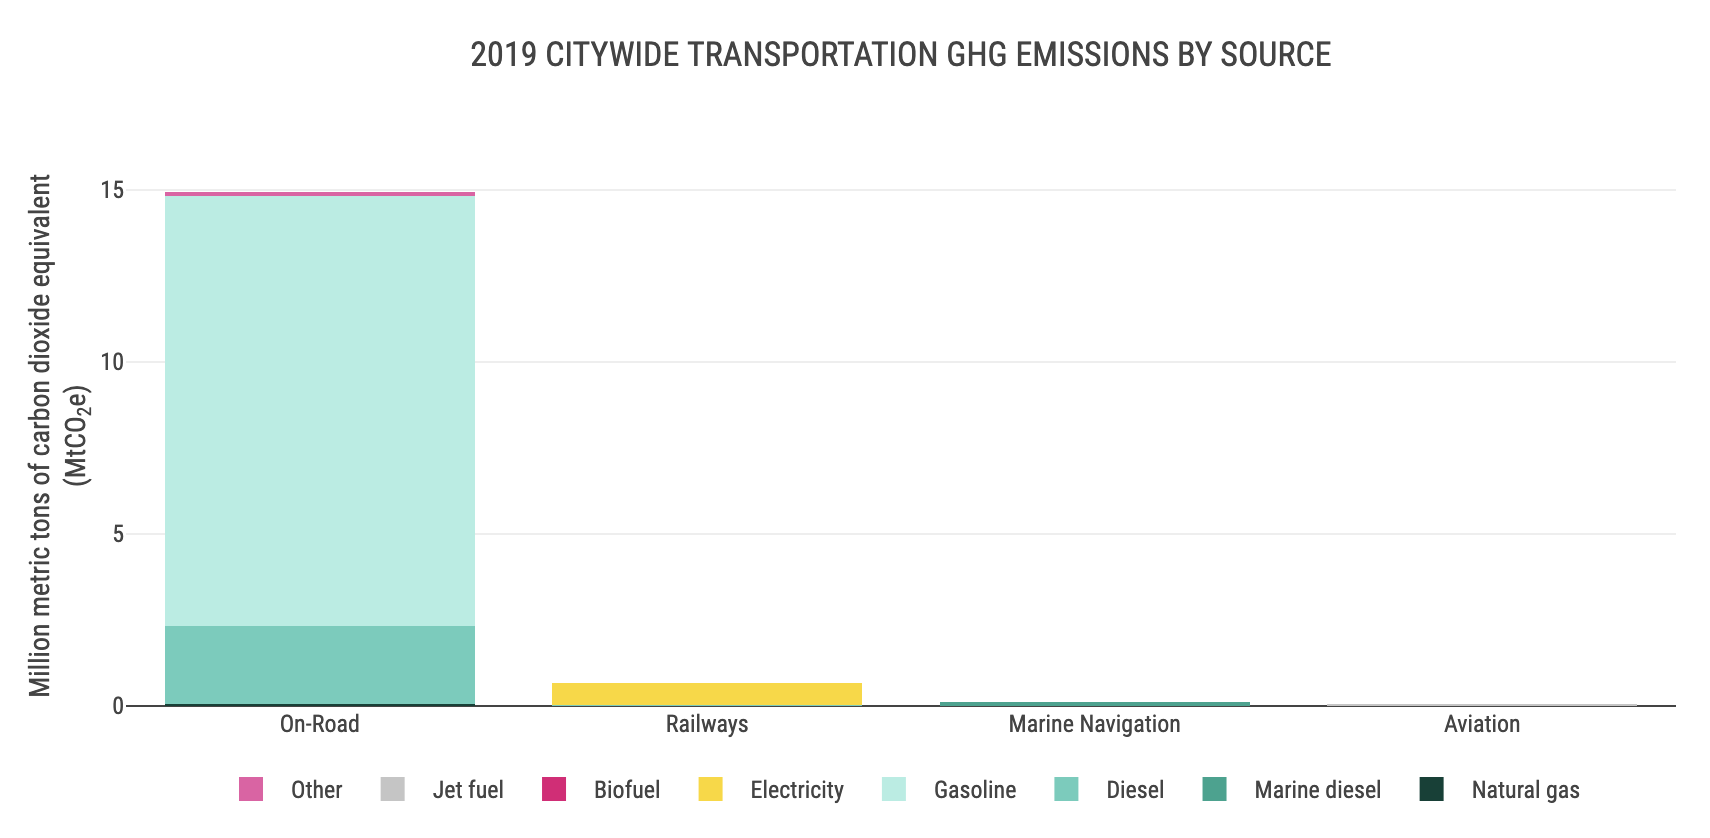
\includegraphics[scale=0.24]{graphics/nyc_ghg_transport.png}

\end{column}
\begin{column}{0.3\textwidth}
\textbf{\color{thickblue}Findings}

\footnotesize
\vspace{1em}

- {\color{lightblue}GHG emissions have reduced 15\%}

- {\color{lightblue}On-road transport is the most remarkable factor for GHG emission in transportation}

\end{column}
\end{columns}


\end{frame}


\begin{frame}
\frametitle{\color{lightred}\textbf{Traffic safety}}
\topline

\textbf{\color{lightred}Crash summary (severity)}

\vspace{1em}

{\centering{
\footnotesize
\begin{tabular}{l|rr|rr} \hline
& \multicolumn{2}{c|}{New York State} & \multicolumn{2}{c}{New York City} \\
& 2015 & 2019 & 2015 & 2019 \\ \hline
Total & 251,142 & 418,687 & 41,632 & 121,091 \\
Fatal & 1,045 & 881 & 232 & 205 \\
Serious & 9,097 & 10,043 & 2,213 & 3,147 \\
Moderate & 15,229 & 16,219 & 4,108 & 5,899 \\
Minor & 75,084 & 85,527 & 24,184 & 35,982 \\
Unk severity & 3,576 & 2,854 & 2,326 & 1,655 \\
Property damage & 147,111 & 303,163 & 8,569 & 74,203 \\
\hline
\end{tabular}
}}


% {\centering{
% \footnotesize
% \begin{tabular}{l|ccccc} \hline
% & Total & Fatal & Serious & Moderate & Minor & Unk \\ \hline
% New York State (2015) & 294,556 & 1,045 & 113,396 & 180,115 \\
% New York State (2019) & 447,021 & 881 & 121,068 & 325,072 \\
% New York City (2015) & \\
% \hline
% \end{tabular}
% }}

    
\end{frame}




\begin{frame}

\frametitle{\color{lightred}\textbf{Travel behavior trend}}
\topline

% \textbf{\color{lightgreen}Drivers of travel}

\begin{columns}
% \hspace{-2em}
\begin{column}{0.5\textwidth}
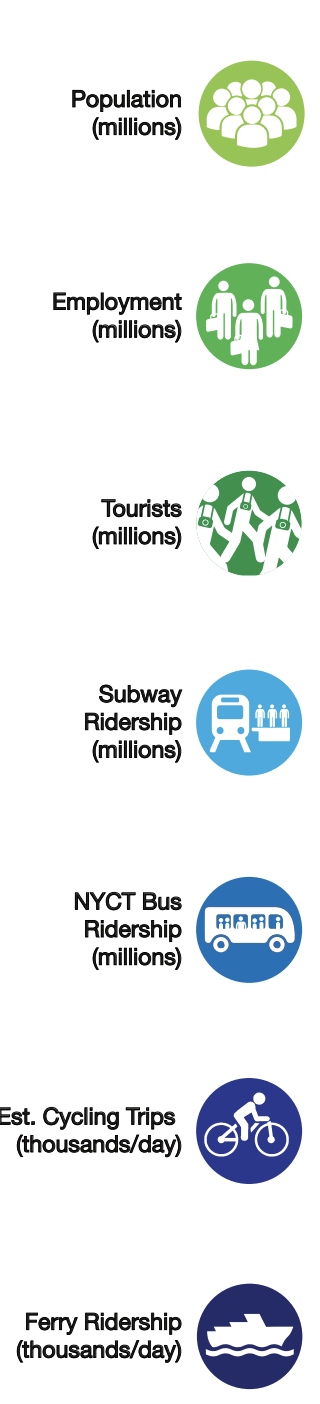
\includegraphics[scale=0.27]{graphics/mobility1.png}\hspace{-0.1em}
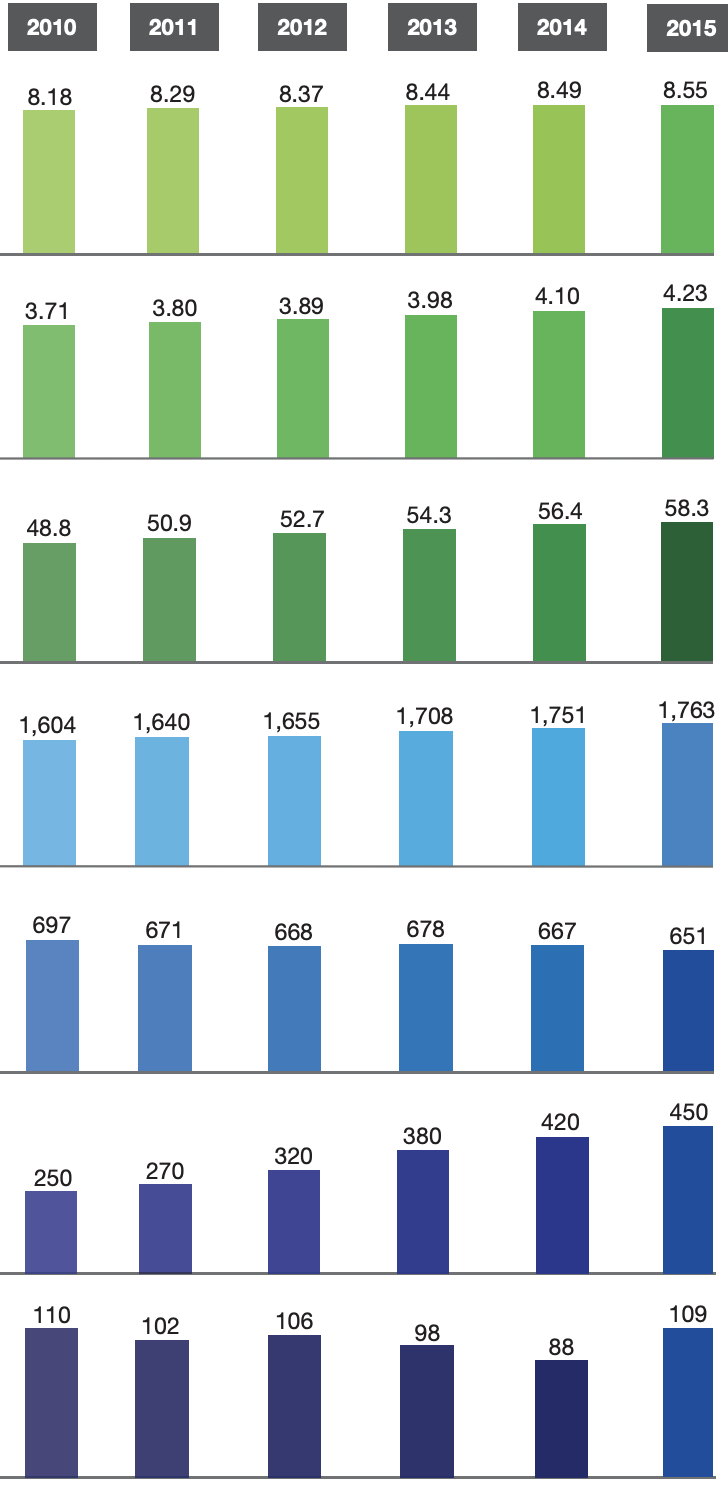
\includegraphics[scale=0.27]{graphics/mobility2.png}
\end{column}

% \hspace{-5em}
\vspace{-15em}
\begin{column}{0.5\textwidth}

% \textbf{\color{thickblue}New York City}

\textbf{\color{lightgreen}Trend}
\begin{itemize}[label=\ding{212}]\footnotesize
    \item \textbf{\color{lightred}Subway ridership} {\color{lightblue}has grown an average of 2\% since 2010}.
    \item \textbf{\color{lightred}Bus rideship} {\color{lightblue}dropped 46 million passengers between 2010 and 2015}.
    \item \textbf{\color{lightred}Cycling} {\color{lightblue}increased by 80\% between 2010 and 2015 as bike infrastructure continued to expand on city streets}.
    \item \textbf{\color{lightred}Ferry ridership} {\color{lightblue}has fluctuated in recent years}.
\end{itemize}
\end{column}
\end{columns}




    
\end{frame}


\begin{frame}

\frametitle{\color{lightred}\textbf{Uniqueness of transport}}
\topline

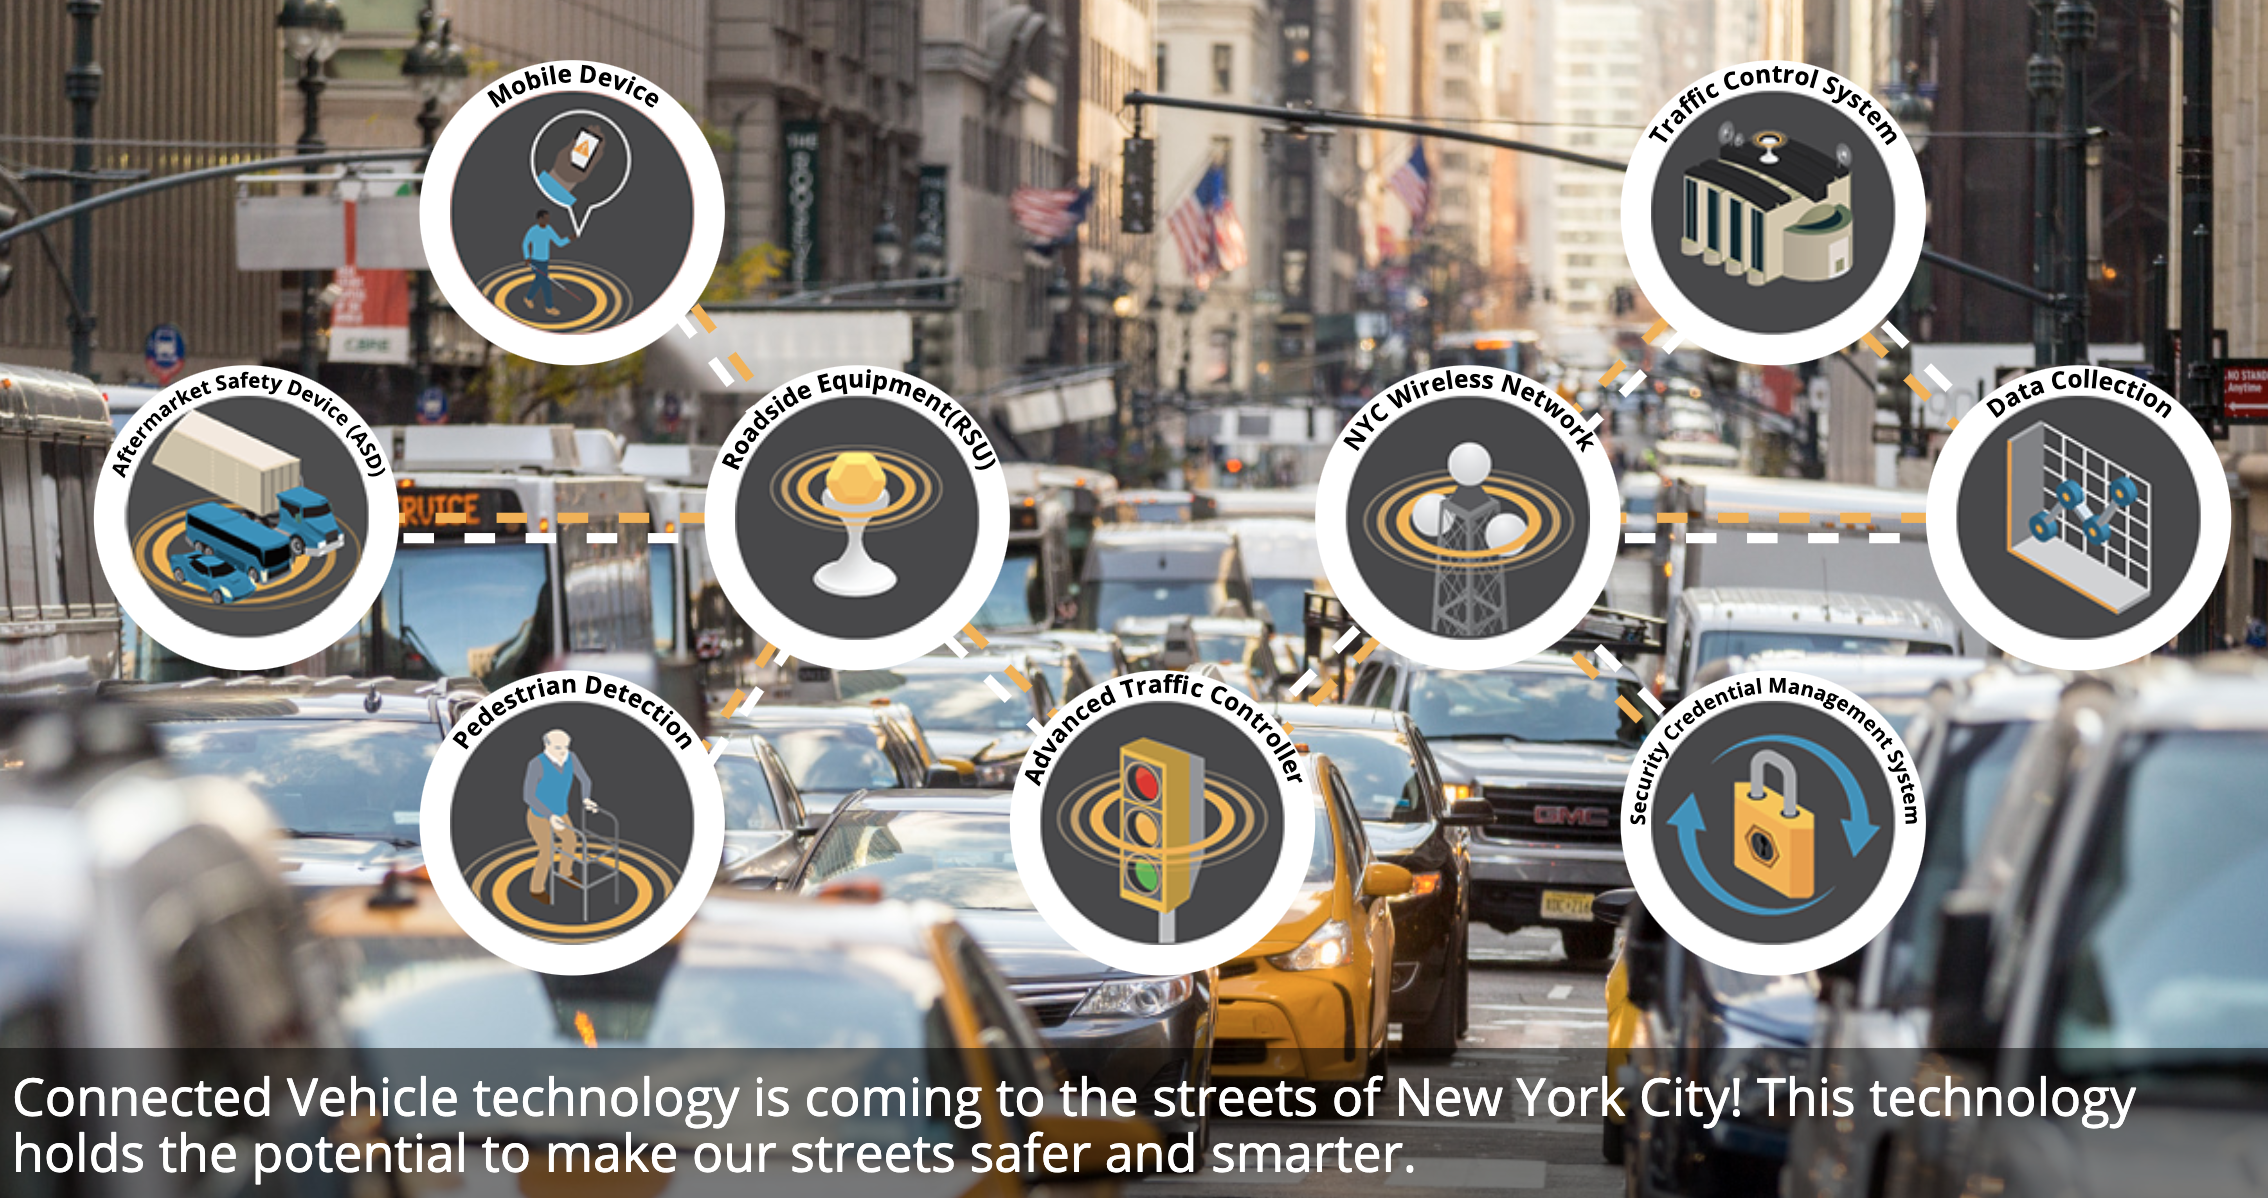
\includegraphics[scale=0.27]{graphics/cv_technology.png}

\vspace{1em}

\footnotesize{New tool to help city {{\color{lightblue}eliminate traffic related deaths}} and {{\color{lightblue}reduce crash related injuries and damage to both the vehicles and infrastructure}}.}

    
\end{frame}




\begin{frame}
\frametitle{\color{lightred}\textbf{Reference}}
\topline

Data and images are taken from:

\footnotesize

\begin{itemize}[label=\ding{48}]
    \item \url{https://www1.nyc.gov/assets/planning/download/pdf/plans/transportation/peripheral_travel_02e.pdf}
    \item \url{https://new.mta.info/agency/new-york-city-transit/subway-bus-ridership-2019}
    \item NYMTC: \url{https://www.nymtc.org/ABOUT-US/annual-reports}
    \item Citi Bike website: \url{https://www.citibikenyc.com/}
    \item Todd W. Schneider (2016). A tale of twenty-two million Citi Bike rides: Analyzing the NYC bike share system. [Blog post]
    \item NYC Connected Vehicle Project: \url{https://www.cvp.nyc/}
    \item ITSMR website: \url{https://www.itsmr.org/sas-guest-portal/}
    \item NYC Taxi \& Limousine Commission (TLC) website: \url{https://www1.nyc.gov/site/tlc/index.page}
    \item Todd W. Schneider (2015). Analyzing 1.1 billion NYC taxi and Uber trips with a vengeance. [Blog post]
    \item GHG emissions: \url{https://nyc-ghg-inventory.cusp.nyu.edu/}
    \item \url{http://tram.mcgill.ca/Teaching/srp/documents/NickC.pdf}
\end{itemize}
    
\end{frame}


\begin{frame}
% \frametitle{\color{black}\textbf{Summary}}
% \topline


\vspace{2em}

\centering\Large {\textbf{\color{lightred}Thanks for your attention!}}
\end{frame}



\end{document}